\subsection{bpmprocess/fft\_\-waveform.c File Reference}
\label{fft__waveform_8c}\index{bpmprocess/fft\_\-waveform.c@{bpmprocess/fft\_\-waveform.c}}


\subsubsection{Detailed Description}


Definition in file {\bf fft\_\-waveform.c}.

{\tt \#include $<$stdio.h$>$}\par
{\tt \#include $<$stdlib.h$>$}\par
{\tt \#include $<$bpm/bpm\_\-messages.h$>$}\par
{\tt \#include $<$bpm/bpm\_\-process.h$>$}\par
{\tt \#include $<$bpm/bpm\_\-dsp.h$>$}\par


Include dependency graph for fft\_\-waveform.c:\nopagebreak
\begin{figure}[H]
\begin{center}
\leavevmode
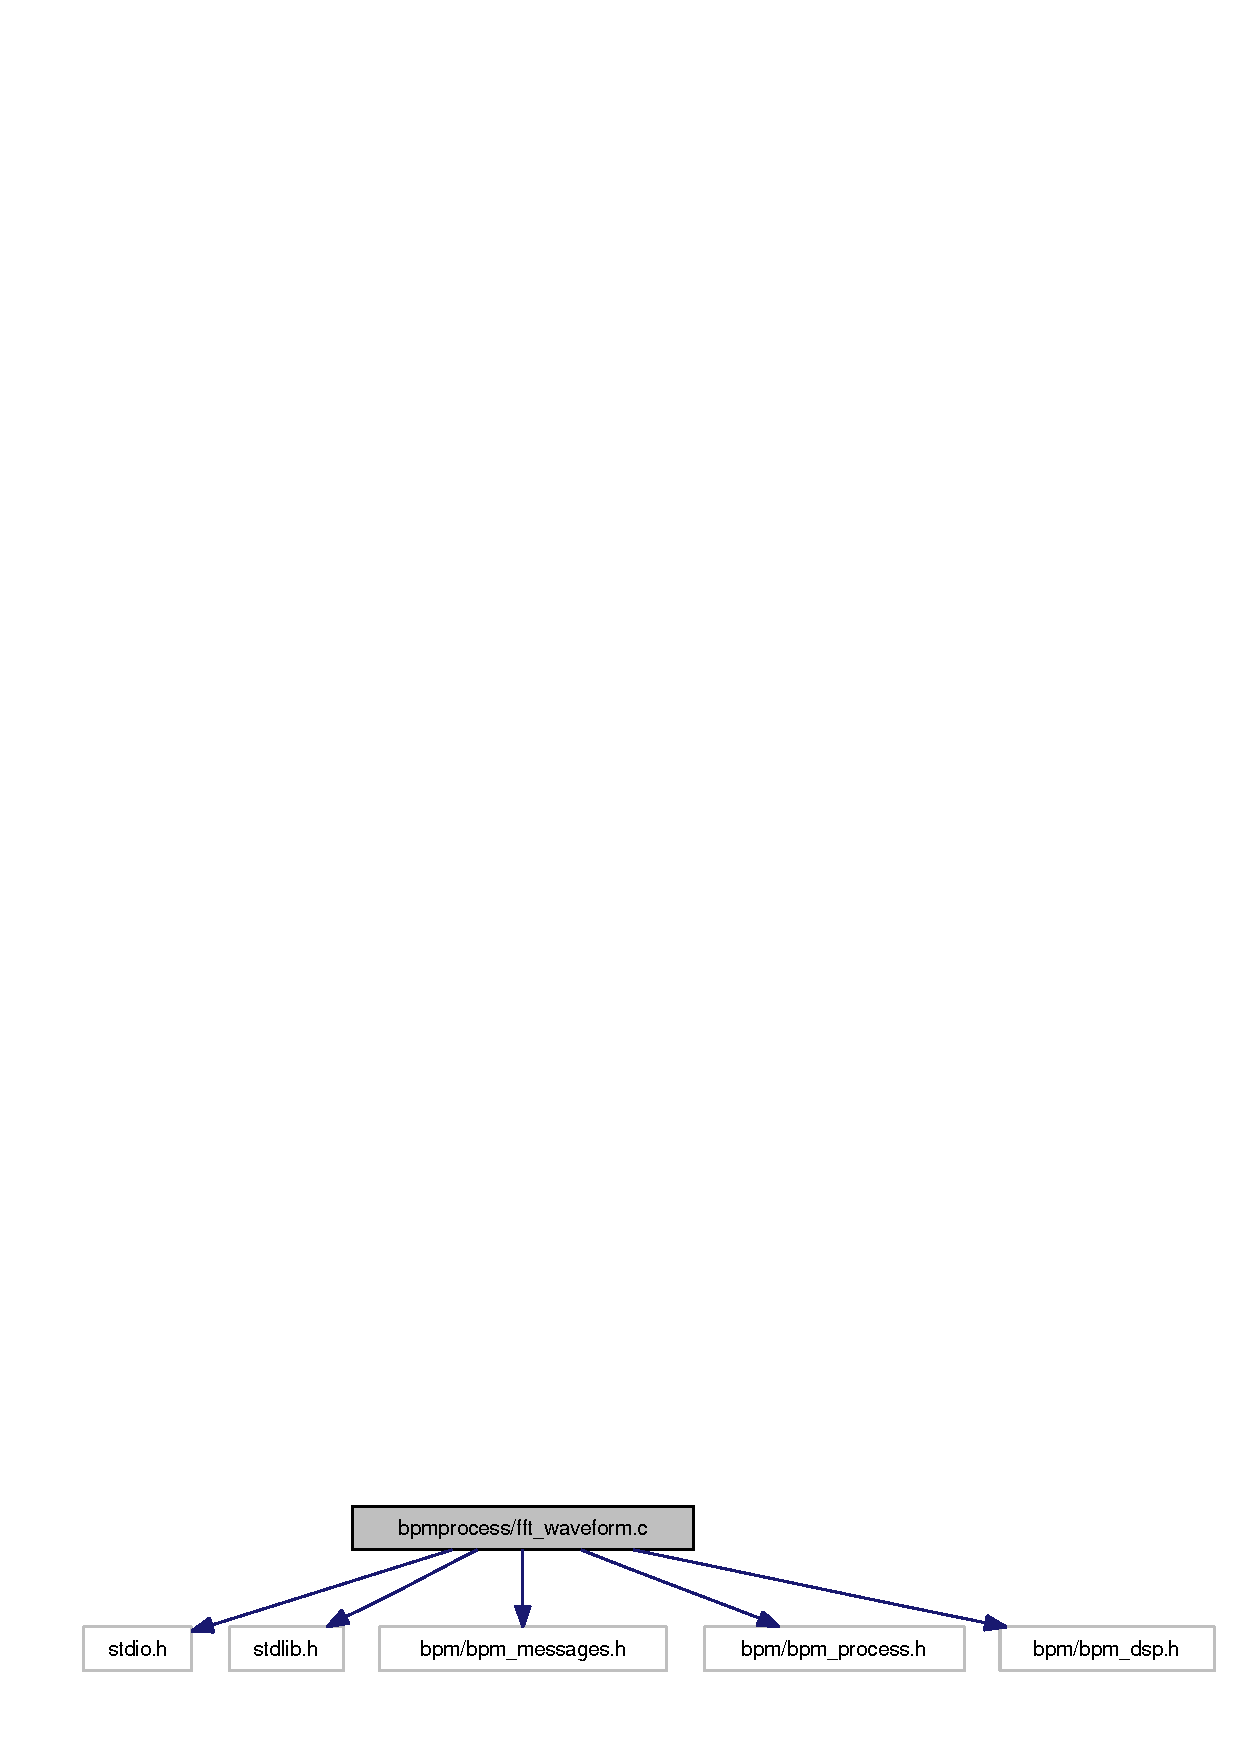
\includegraphics[width=293pt]{fft__waveform_8c__incl}
\end{center}
\end{figure}
\subsubsection*{Functions}
\begin{CompactItemize}
\item 
int {\bf fft\_\-waveform} ({\bf doublewf\_\-t} $\ast$w, {\bf complexwf\_\-t} $\ast$fft)
\end{CompactItemize}
